\section{Introduction}
\label{sec:intro}

Molecular representation learning, which automates the process of feature learning for molecules, is fast driving the development of computational chemistry and drug discovery. It has been recognized as crucial for a variety of downstream tasks, spanning from molecular property prediction to molecule design \cite{Yang:2019al,Du:2022ek}.
Deep neural models, on the other hand, rely on a substantial amount of labeled data, which require expensive wet lab experiments in chemical domains.
With insufficient annotated data, deep models easily overfit to such small training data and tend to learn spurious correlations \cite{Sagawa:2020we}.

In recent years, self-supervised pretraining has emerged as a promising strategy to alleviate the label scarcity problem and improve model robustness \cite{Jing:2021cf}.
A typical framework pretrains the encoder model with training objectives over large-scale unlabeled datasets and then fine-tunes the learned model on labeled downstream tasks.
Motivated by its success, many molecular pretraining models have been developed \cite{Wang:2019hp,Chithrananda:2020eo,Hu:2020uz,You:2020ut,Xu:2021tv,Fang:2022et,Stark:2021ug,Liu:2022vr}.
To capture chemical semantics of molecules, these models design several pretraining strategies based on different \emph{molecular featurizations}, which translate chemical information into representations that can be recognized by machine learning algorithms.
For example, early models \cite{Wang:2019hp,Chithrananda:2020eo} propose to leverage masked language modeling \cite{Bengio:2003vh} to pretrain Simplified Molecular-Input Line-Entry System (SMILES) strings \cite{Weininger:1988sm}, while others study contrastive learning on 2D graphs \cite{Hu:2020uz,You:2020ut,Xu:2021tv} or 3D conformations \cite{Fang:2022et}.
Some recent studies further propose to enrich 2D-topology-based pretraining with 3D geometry information \cite{Stark:2021ug,Liu:2022vr}.

Despite encouraging progress, prior studies tend to emphasize on pretraining on molecular graphs and overlook the impact of other molecular featurizations with their corresponding neural encoders, which represent chemical information in different ways.
Consider SMILES strings as an example. It explicitly represents informative structures in special characters such as branches, rings, and chirality \cite{Ross:2022hh}, which are difficult to learn in graph-based representations \cite{Chen:2020vz}.
Moreover, the utility of different featurizations may vary across downstream tasks. Therefore, most previous models relying on only one or two featurizations might achieve sub-optimal performance across various downstream tasks.
For example, 2D topology is important for many drug-related properties such as toxicity, while 3D geometry arguably determines properties related to quantum mechanics, such as single-point energy, atomic forces, or dipole moments \cite{Zhang:2018dp,Smith:2017an}.
Therefore, it is natural to ask whether we can enjoy the benefits from multiple molecular featurizations and take the relative utilities of different featurizations into consideration during fine-tuning on downstream tasks.

\begin{figure}
	\centering
	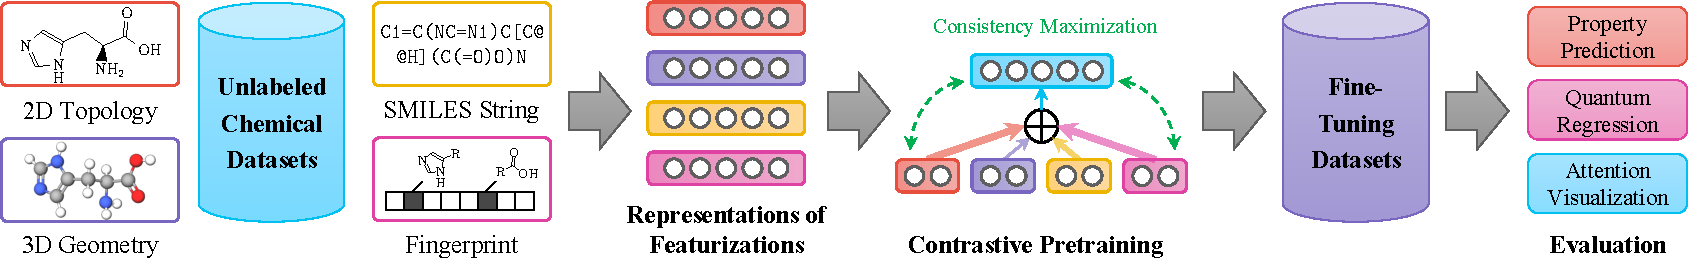
\includegraphics[width=\linewidth,bb=0 0 811 132]{figures/model.pdf}
	\caption{The proposed \themodel model. \themodel obtains four molecule featurizations with appropriate encoders. After that, an attention network is employed to aggregate each view embedding and compute a final embedding. The model is trained using a contrastive objective that maximizes the consistency between view embeddings and the final embedding.}
	\label{fig:model}
\end{figure}

In this work, we first revisit four commonly used featurizations techniques: (a) 2D topology graphs, (b) 3D geometry graphs, (c) Morgan fingerprints, and (d) SMILES strings.
We leverage four accompanying neural encoders with proper inductive bias and conduct two case studies, classifying tetrahedral chiral centers and counting aromatic rings, both of which are informative chemical descriptors, on representations obtained on different featurization techniques.
The results show there is no one single featurization that dominates the others, indicating that different featurizations encode chemical semantics of molecules in different ways.

In light of this observation, we then propose a simple and effective \underline{MO}lecular pretraining framework with \underline{CO}mplementary featurizations to comprehensively leverage every featurization during both pretraining and fine-tuning, which we term \themodel for brevity.
Its graphical illustration is shown in \cref{fig:model}.
The core idea of \themodel is to dynamically adjust the contribution of each featurization through an attention network, which \emph{selectively} extracts information from each complementary ``view'' of the raw molecular data.
Besides, we design a novel multiview contrastive pretraining strategy, which trains the model by maximizing the consistency among different views in a self-supervised manner.
Contrary to previous studies \cite{Stark:2021ug,Liu:2022vr} that only consider 2D graph structures during fine-tuning, our \themodel utilizes multiple featurizations in \emph{both} pretraining and fine-tuning stages and further allows interpretation analysis of different downstream tasks for domain scientists.
Note that our proposed \themodel framework is generic, allowing for seamless integration of off-the-shelf neural architectures.
To the best of our knowledge, this is the first work that studies how various featurization techniques should be utilized for molecular pretraining and downstream tasks.

We evaluate the effectiveness of our \themodel model on widely-used benchmark datasets including MoleculeNet \cite{Wu:2018dv} and QM9 \cite{Ramakrishnan:2014ij} that cover a wide range of molecular property prediction tasks.
The results reveal that \themodel consistently improves non-pretraining baselines without negative transfer and outperforms existing state-of-the-art molec ular pretraining models, achieving a 1.1\% absolute improvement in terms of average ROC-AUC.
Furthermore, the learned model weights of molecular featurizations for different end tasks are well aligned with prior chemical knowledge.
We also suggest a series of guidelines on choosing effective featurization techniques for molecular representations.

The main contributions of this work are three-fold:
\begin{itemize}
	\item We explore the featurization spaces of molecules with appropriate neural encoders and highlight the importance of incorporating different featurizations for molecular pretraining.
	\item We propose a novel molecular contrastive pretraining framework that adaptively integrates information from multiple complementary featurizations during both pretraining and fine-tuning stages and provides interpretability for downstream molecular property prediction tasks.
	\item Extensive experiments conducted on public benchmark datasets validate the effectiveness of our proposed model. \themodel is able to achieve the state-of-the-art across various downstream datasets without negative transfer.
\end{itemize}
